\chapter{ElmerGrid Interface Examples}

\section{Ansys mesh to Elmer}

The APDL macros and the following documentation have been written
by {\em Antti Pursula} (email: Antti.Pursula@csc.fi). He will 
answer any further questions related to the macros.

Two APDL (Ansys parametric design language) macros has been created
which allow writing geometry data in ASCII format out of Ansys. The
macros can be activated from Ansys GUI using custom added buttons in
the Ansys Toolbar. The ASCII format files can further be converted in
the Elmer format by using ElmerGrid.

The information written out by the macros consists of four files that
are named \texttt{ExportMesh.*} (\texttt{* = header, node, elem}, or
\texttt{boundary}). The files include all the information Elmer needs for using
the mesh ie., besides the obvious node and element definitions, also
information about the boundary nodes. 

%Detailed information of the file
%formats is found here (in Finnish), but this information is not needed
%in any way when using Ansys to Elmer interface.

In Ansys, the geometry model is often created combining several
elementary geometries. This means that the model usually includes
boundaries, that have no physical meaning. These do not disturb the
analysis neither in Ansys nor in Elmer, but they can make the
definition of boundary conditions quite cumbersome in
Elmer. Therefore, there are two possible macros for exporting data
from Ansys: ELMER\_AU and ELMER\_CH. The first writes all the boundaries
of the model automatically while the second asks the user to
graphically pick the boundaries that have physical meaning. It is
worthwhile to notice that Elmer does not necessarily need boundary
information for all the physical boundaries, but only those on which a
boundary condition is to be applied.

To use Ansys to Elmer interface you need to download two macro files
and an Ansys start-up file and copy them into your working
directory. After the files have been copied, start Ansys and the
buttons ELMER\_AU and ELMER\_CH appear in the Toolbar. The conversion of
the resulting ASCII files into Elmer format is done by the ElmerGrid
program. The files as well as ElmerGrid can be downloaded from the
Elmer download page.

%ElmerGrid is controlled through command line arguments. 
%
%The syntax is
%ElmerGrid input\_format output\_format filename [options]. The input and
%output formats are numbers. 
%
In ElmerGrid the Ansys input format is 4 and output
format can be Elmer mesh format (3) or ElmerPost format (2). So,
creating Elmer meshes from Ansys input is done with the command:
\texttt{ElmerGrid 4 3 ExportMesh}. There are also many command-line 
options available. The
most important ones in this case are:
%
\begin{itemize}
  \item \texttt{-o name} for saving output with the name specified.  
  \item \texttt{-order $c_x$ $c_y$ $c_z$} for reordering nodes and elements using $c_1x+c_2y +c_3z$.  
  \item \texttt{-scale $c_x$ $c_y$ $c_z$} for scaling the mesh using the constant to multiply
the coordinate values.
  \item \texttt{-merge epsilon} for merging nodes that are at most distance epsilon apart.
\end{itemize}

The \texttt{-merge} option is important in a case where Ansys creates multiple
nodes on a boundary of two elementary geometries. These nodes are
often noticed only when Elmer is not able to use a mesh created from
Ansys. In such a case, use \texttt{-merge} option with a suitable value 
for the node separation.

\begin{figure}
\begin{center}
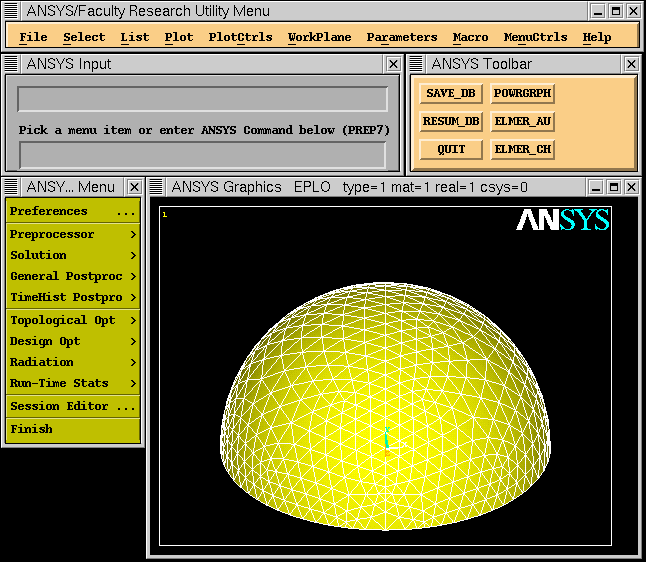
\includegraphics[height=5cm]{ansys2elmer-a}
\hspace{10mm}
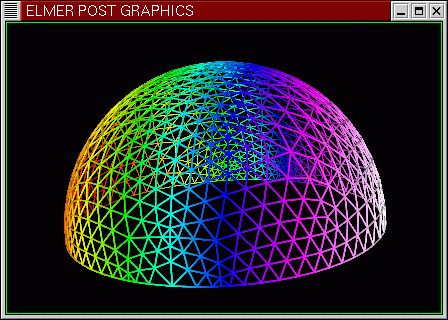
\includegraphics[height=5cm]{ansys2elmer-b}
\end{center}
\caption{Pictures of the same mesh in Ansys desktop and in ElmerPost window.}
%\label{pic5}
\end{figure}


\section{Comsol Multiphysics (Femlab) mesh to Elmer}

Comsol Multiphysics is a widely used finite element tool with highly 
automated mesh generation. Previously the software was known as Femlab. 
There are two different strategies depending whether one uses the old or new
version. 
The ElmerGrid utility tries first to apply the Comsol Multiphysics strategy and then
uses the older Matlab version. 


\subsection{Comsol Multiphysics with pmhtxt-export}

In the older versions of Comsol Multiphysics/Femlab there 
wasn't any export format that would have included the boundary definitions. 
However, since version 3.2 of Comsol Multiphysics there 
is a suitable export format that may be directly used to export meshes in Elmer. 
The ElmerGrid program 
understands a sufficient subset of the commands in mphtxt-file of 
Comsol multiphysics. 

The procedure for importing meshes to Elmer is
\begin{itemize}
  \item In Comsol Multiphysics choose \\
   \texttt{File -> Export -> Mesh to File}
   \item Select the export format \\ \texttt{``COMSOL Multiphysics text file'' (mphtxt)}
   \item Give the mesh a file name, e.g. \texttt{mymesh} and you obtain the 
    file \texttt{mymesh.mphtxt}
  \item Call then ElmerGrid with the following command line options \\
    \texttt{ElmerGrid 9 2 mymesh.mphtxt}
\end{itemize}
As a result you get a directory \texttt{mymesh} which may be used in Elmer 
computations. The utility should be backward compatible for some time.


\subsection{Femlab version bundled with Matlab}

The original version of Femlab was bundled with 
Matlab and therefore a natural approach to export results from Femlab was 
to use a .m script that provided all the necessary information. 
The mesh export strategy is applicable for 2D and 3D meshes consisting
of triangles, and for 3D tetrahedral meshes. It is not possible to
combine volume and surface meshes unless the surface is part of the
volume mesh. The needed export utility for Femlab/Matlab is obtained from
the Elmer download page

The export is performed in following steps:
\begin{enumerate}
\item When you have created a mesh in Femlab choose \texttt{Export to
Workspace} and thereafter \texttt{Mesh}. The suggested name is \texttt{mesh}, but that
may be changed.  
%
\item Then go to Matlab and run the provided 
command-file \texttt{savemesh.m}. The only parameter is the name of the mesh
data, e.g. \texttt{savemesh(mesh)}. This command then creates files \\
FemlabMesh.header: information of vector sizes  \\
FemlabMesh.node: node coordinates  \\
FemlabMesh.elem: element topologies  \\
FemlabMesh.boundary: boundary side definitions  
%
\item To transform the mesh for a format known by
Elmer use ElmerGrid. The flag for Femlab export format is 9. Use the
following commands:  \\
\texttt{ElmerGrid 9 2 meshname}: for making mesh files
usable by ElmerFront and ElmerSolver  \\ 
\texttt{ElmerGrid 9 3 meshname}: For viewing the mesh with ElmerPost  
You may also use many ElmerGrid
options, such as \texttt{-order real[3]} 
where the vector orders the nodes to
decrease the matrix bandwidth, e.g. \texttt{ElmerGrid 9 2 meshname -out outname
-order 1.0 2.0 3.0}
\end{enumerate}

\begin{figure}
\begin{center}
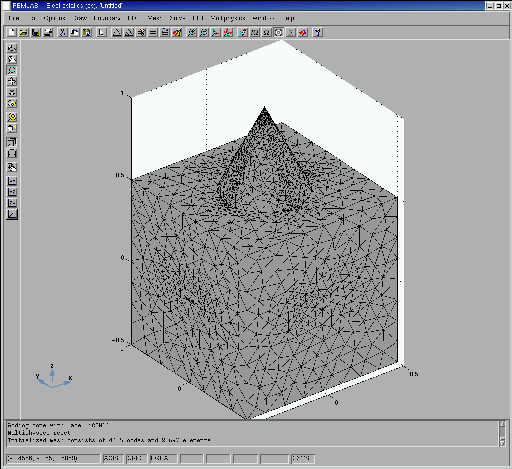
\includegraphics[height=5cm]{femlab2elmer-a}
\hspace{10mm}
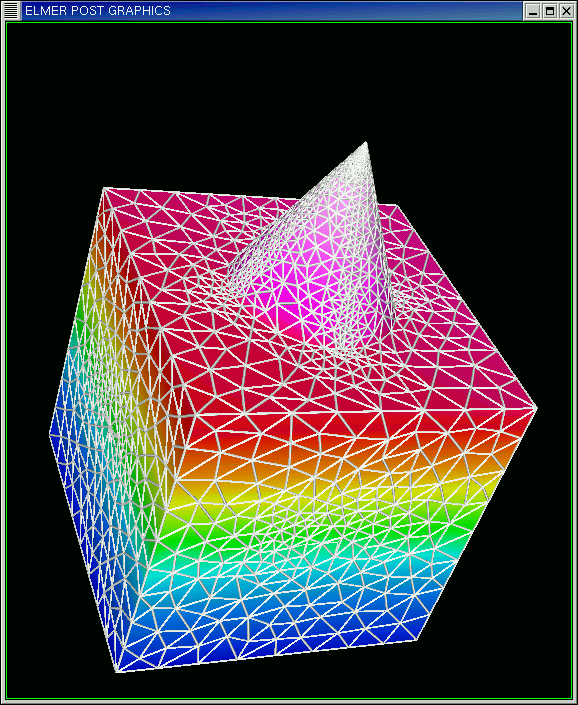
\includegraphics[height=5cm]{femlab2elmer-b}
\end{center}
\caption{Pictures of the same mesh in Femlab desktop and in ElmerPost window.}
%\label{pic5}
\end{figure}


\section{Triangle mesh to Elmer}

Triangle is a two-dimensional quality mesh generator and Delaunay triangulator.
written by Jonathan Richard Shewchuk
in University of California at Berkeley (email: jrs@cs.berkeley.edu).

The format written by Triangle is very similar to that one needed by Elmer. 
The only problem is to find the boundaries defined by the nodes known
to lie on the boundary. The current implementation of the algorithm may
result to problems at the corners. Also the functionality hasn't been tested for
cases with several materials or several boundaries.

Assuming we have a triangle input file name \texttt{tri.poly}. This may be meshed 
with second order triangles having all corners above 32.0 degrees and 
area below 0.001 with the command
\begin{verbatim}
triangle -pq32.0 -a.0001 -o2 tri
\end{verbatim}
\noindent This creates files \texttt{tri.i.ele} and \texttt{tri.i.node}
 (i=$1,2,\ldots$),
which may be used to create the Elmer model.

The Triangle format corresponds to input mode 11 at ElmerGrid. Therefore
the mesh for ElmerSolver is created with command
\begin{verbatim}
ElmerGrid 11 2 tri.1
\end{verbatim}
\noindent
which results to a computational mesh being saved at ElmerSolver format in
subdirectory \texttt{tri}.

\begin{figure}
\begin{center}
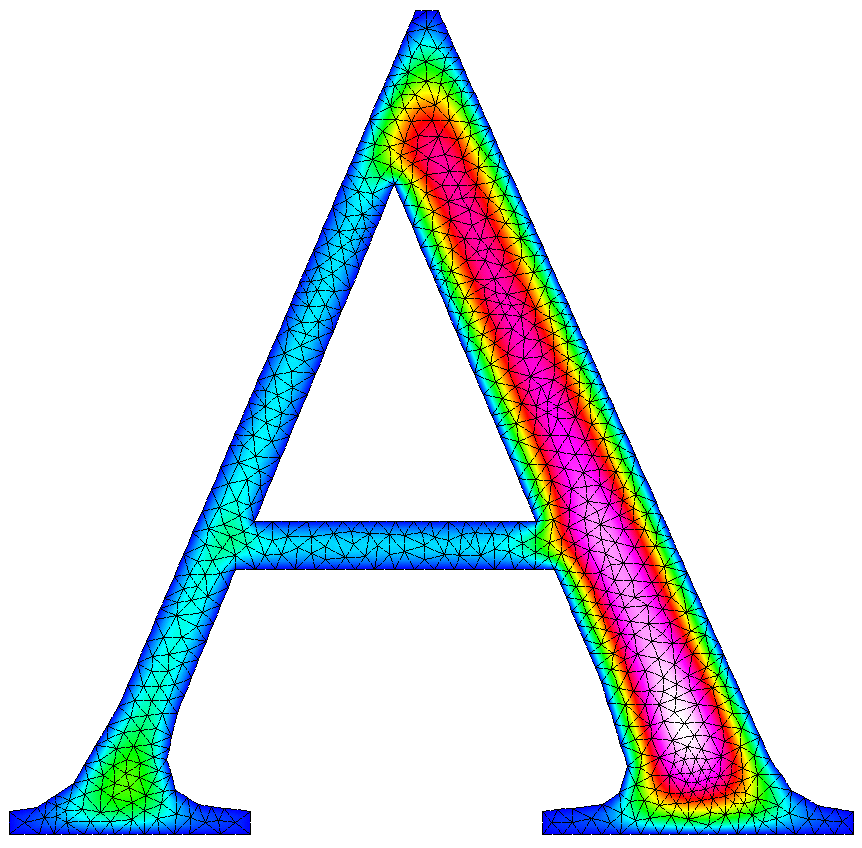
\includegraphics[height=5cm]{triangle2elmer}
\end{center}
\caption{Picture of the Triangle example case in ElmerPost.}
%\label{pic5}
\end{figure}


